\documentclass[11pt, a4paper]{article}

% ---------- Paquetes ----------
\usepackage[a4paper, margin=2.5cm]{geometry}
\usepackage[english]{babel}
\usepackage{graphicx}
\usepackage{amsmath}
\usepackage{float}
\usepackage{parskip}
\usepackage[svgnames]{xcolor}
\usepackage{titlesec}
\usepackage{fancyhdr}
\usepackage{enumitem}
\usepackage{hyperref} % hyperref se carga al final

% ---------- Configuración ----------
\setlength{\headheight}{14pt}
\graphicspath{{./}{figures/}{../figures/}} % ajusta a tu estructura de carpetas

% Set up custom heading colors
\titleformat{\section}{\Large\bfseries\color{Black}}{\thesection}{1em}{}
\titleformat{\subsection}{\large\bfseries\color{Black}}{\thesubsection}{1em}{}

% Set up clean header and footer
\pagestyle{fancy}
\fancyhf{}
\fancyhead[L]{\textcolor{gray}{\small Statistical Physics Lab 1}}
\fancyhead[R]{\textcolor{gray}{\small Group Team Name}}
\fancyfoot[C]{\thepage}
\renewcommand{\headrulewidth}{0.4pt}

\begin{document}

\begin{flushleft}
{\Huge \bfseries \color{Black} Microstates and Macroscopic Thermodynamics of a Binary System \par}
\vspace{0.5em}
{\Large \color{DarkGray} Statistical Physics Laboratory Practice 1 \par}
\vspace{1.5em}
{\large
\textbf{Group Team Name / ID} \\
Author 1 (NIA: 100553552, GitHub: @asierrrrrrr) \\
Author 2 (NIA: 100507899, GitHub: @manojantony147-bot) \\
Author 3 (NIA: 100551012, GitHub: @dariovalero) \\
Author 4 (NIA: 100550907, GitHub: @jorgesck777)
\par}
\vspace{1em}
\textcolor{gray}{November 4, 2026 \quad|\quad Department of Physics, Universidad Carlos III de Madrid}
\end{flushleft}

\vspace{0.5em}
{\color{Black}\hrule height 1.5pt}
\vspace{1.5em}

\begin{abstract}
This report investigates the statistical mechanics of a system composed of independent
binary elements (unbiased coins) as an exact computational and physical model for discrete
two-state assemblies. We present a modular Python implementation that enumerates microstates,
calculates binomial distribution frequencies using log-space arithmetic to prevent
numerical overflow, and explores scaling behavior as $N\rightarrow10^{23}$. Additionally, we derive state
probabilities, compute Boltzmann entropy variations $\Delta S$, and analyze the thermodynamic
limit and micro-reversibility in connection with the Second Law of Thermodynamics.
\end{abstract}

\noindent \textbf{Repository Link:} \url{https://github.com/manojantony147-bot/StatPhys_Lab1_GroupD}

\vspace{2em}

\tableofcontents

\newpage

\section{Introduction \& Objectives}
The primary objective of this practice is to investigate the microscopic configurations and macroscopic properties of a system composed of independent, unbiased binary elements, computationally modeled as unloaded coins. Although conceptually simple, this binary model serves as a foundational and exact analog for numerous physical systems whose constituent elements can be described by two possible states. 

By evaluating the total number of possible microscopic configurations and grouping them by their measurable macroscopic quantities (macrostates), we calculate the corresponding binomial probability distribution:
\begin{equation}
\Omega(N,k)=\binom{N}{k}=\frac{N!}{k!(N-k)!}
\end{equation}

Furthermore, this exercise explores the extrapolation of these statistical mechanics principles to large system sizes, calculating the transition towards the macroscopic thermodynamic limit ($N \sim 10^{23}$). By explicitly connecting the statistical multiplicity of these states to the Boltzmann entropy equation ($S = k_B \ln \Omega$), this report aims to givr a rigorous statistical foundation for the Second Law of Thermodynamics, demonstrating how macroscopic irreversibility comes from pure statistical probabilities.
\section{Methodology \& Collaborative Workflow}
\subsection{Environment \& Reproducibility}
The computational environment was configured using Miniconda (\texttt{Python 3.11}). All dependencies are specified in \texttt{environment.yml} to guarantee cross-platform execution reproducibility.

\subsection{Version Control \& Repository Architecture}
Collaborative development was managed via GitHub using a Feature-Branch workflow. Code reviews were required before merging Pull Requests into the \texttt{main} branch. The repository layout follows a modular Python structure:

\begin{itemize}
    \item \texttt{src/}: Modular logic for microstate iteration, combinatorics, and entropy calculation.
    \item \texttt{tests/}: Automated unit tests built with \texttt{pytest}.
    \item \texttt{notebooks/} \& \texttt{report/}: Exploratory plots and LaTeX source.
\end{itemize}

\section{Computational Analysis of Microstates}
All the tests performed in this section can be seen in \texttt{microstates\_tests.py}.

\subsection{Enumeration for $N=7$}
For a system of $N=7$ coins, there are a total of $\Omega_{total} = 2^7 = 128$ possible microstates. After a computational enumeration was carried out, the whole 128 unique binary sequences from $(0, 0, 0, 0, 0, 0, 0)$ to $(1, 1, 1, 1, 1, 1, 1)$ were obtained. Grouping these microstates by their corresponding macrostate (defined by the number of heads, $k$) yields the binomial distribution shown in Table \ref{tab:n7_macrostates}.

\begin{table}[H]
    \centering
    \begin{tabular}{cc}
        \hline
        \textbf{Macrostate ($k$ heads)} & \textbf{Number of Microstates ($\Omega$)} \\
        \hline
        0 & 1 \\
        1 & 7 \\
        2 & 21 \\
        3 & 35 \\
        4 & 35 \\
        5 & 21 \\
        6 & 7 \\
        7 & 1 \\
        \hline
        \textbf{Total} & \textbf{128} \\
        \hline
    \end{tabular}
    \caption{Number of microstates for each macrostate in a system of $N=7$ coins.}
    \label{tab:n7_macrostates}
\end{table}

\subsection{Full Enumeration Limit ($2^{N}$)}
Based on the 5-minute wall-clock benchmark, the largest system size that our program can fully enumerate is \textbf{$N = 26$}, which is completed in 306.43 seconds.

The principal limiting factor we have encountered for the full enumeration is the computational time complexity, which increases exponentially as $\mathcal{O}(2^N)$. Each time $N$ increases by 1, the number of possible microstates doubles, doubling as well the number of required CPU cycles to perform the operations (as an example, $N=24$ took $\sim$69s, $N=25$ took $\sim$152s, and $N=26$ took $\sim$306s). The memory has not been a limiting factor, since a Python generator was used, which provides one state at a time instead of storing all $2^N$ arrays in memory. As shown in the benchmark, memory usage remained  constant at $\sim$0.001 MB throughout the execution, proving that CPU time (not RAM) is the determining obstacle for the enumeration of high values of N.

\subsection{Macrostate Frequency Distributions ($N=20,50,80,100$)}

 For $N \in \{20, 50, 80, 100\}$, the macrostate frequencies were computed for all $k \in [0, N]$. As $N$ increases, the absolute number of microstates for the most probable macrostate ($k = N/2$) grows vastly. As shown in Figure \ref{fig:macrostate_distributions}, the discrete binomial distributions converge toward a Gaussian bell curve centered at $N/2$, illustrating how the distribution becomes more and more concentrated around the mean as the system size grows.

\begin{figure}[H]
    \centering
    % Top row: N=20 and N=50
    \begin{minipage}{0.48\textwidth}
        \centering
        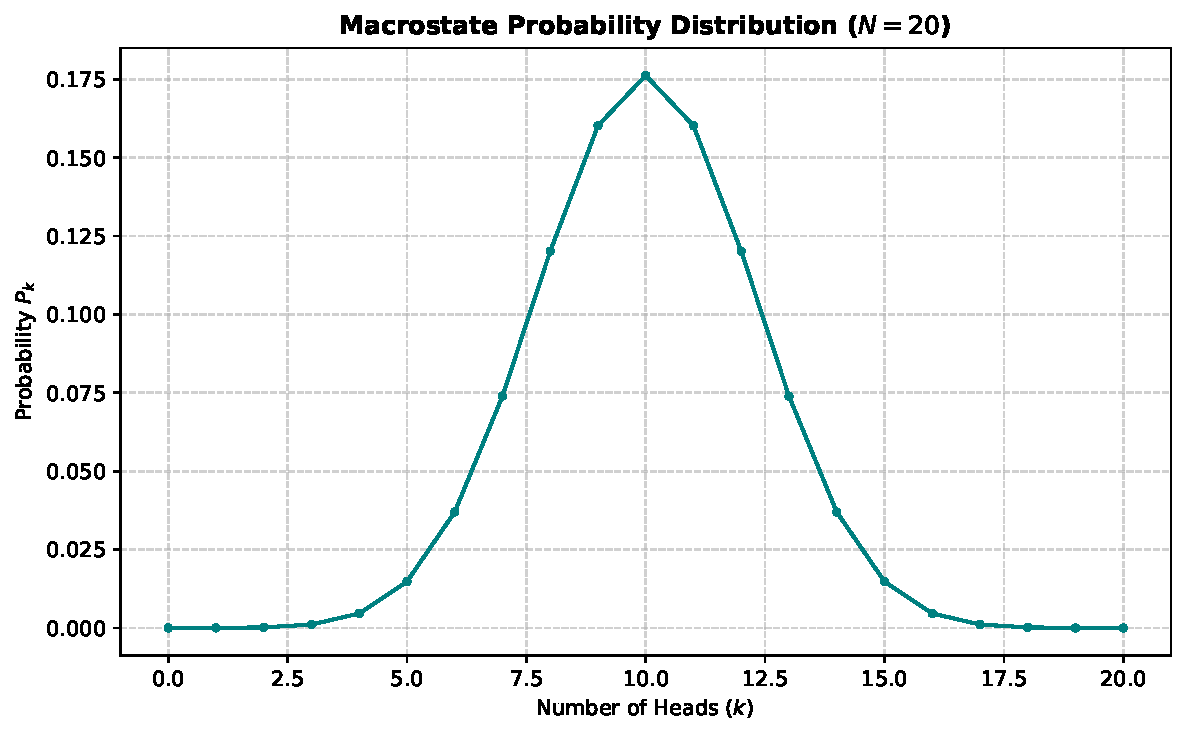
\includegraphics[width=\linewidth]{probability_distribution_N20.pdf}
    \end{minipage}\hfill
    \begin{minipage}{0.48\textwidth}
        \centering
        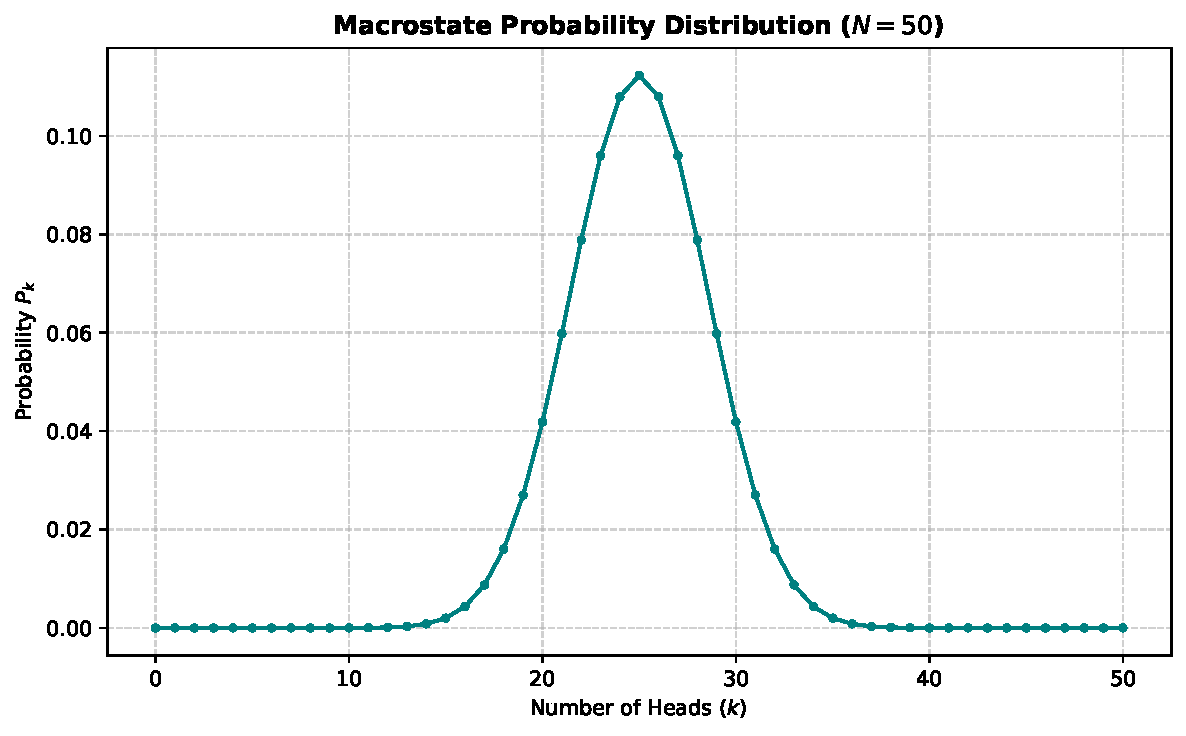
\includegraphics[width=\linewidth]{probability_distribution_N50.pdf}
    \end{minipage}

    \vspace{0.4cm} % Adds a bit of space between rows

    % Bottom row: N=80 and N=100
    \begin{minipage}{0.48\textwidth}
        \centering
        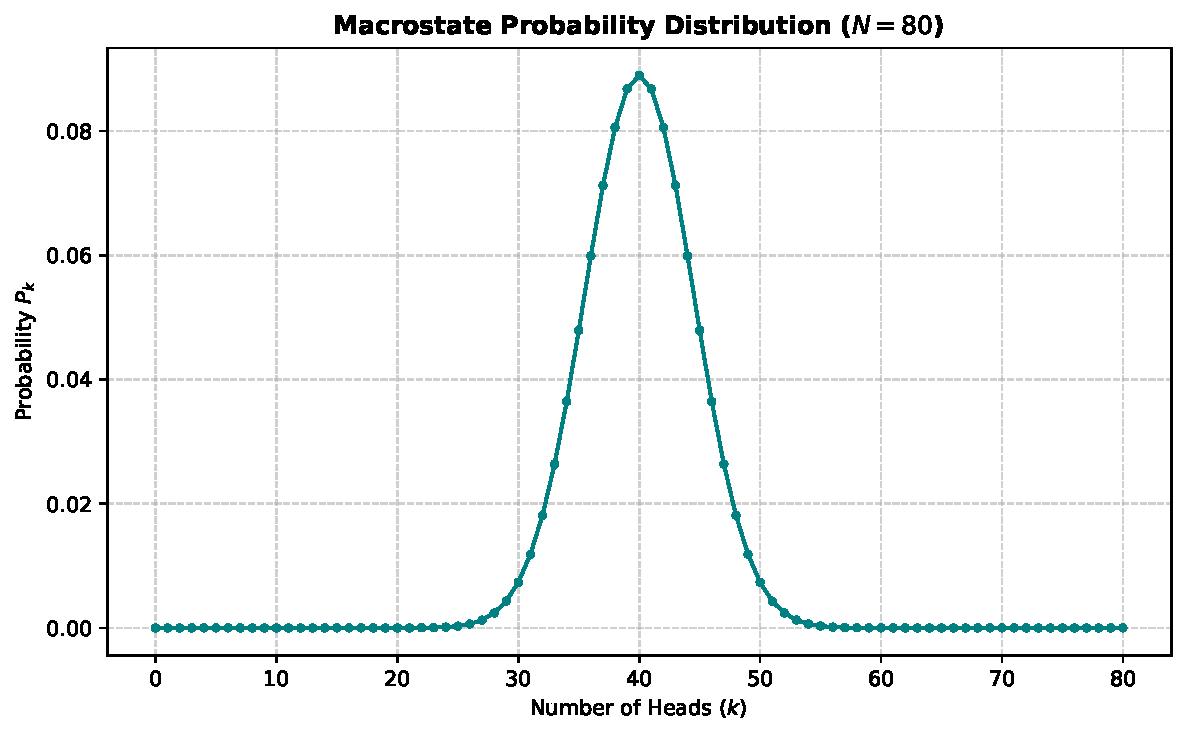
\includegraphics[width=\linewidth]{probability_distribution_N80.pdf}
    \end{minipage}\hfill
    \begin{minipage}{0.48\textwidth}
        \centering
        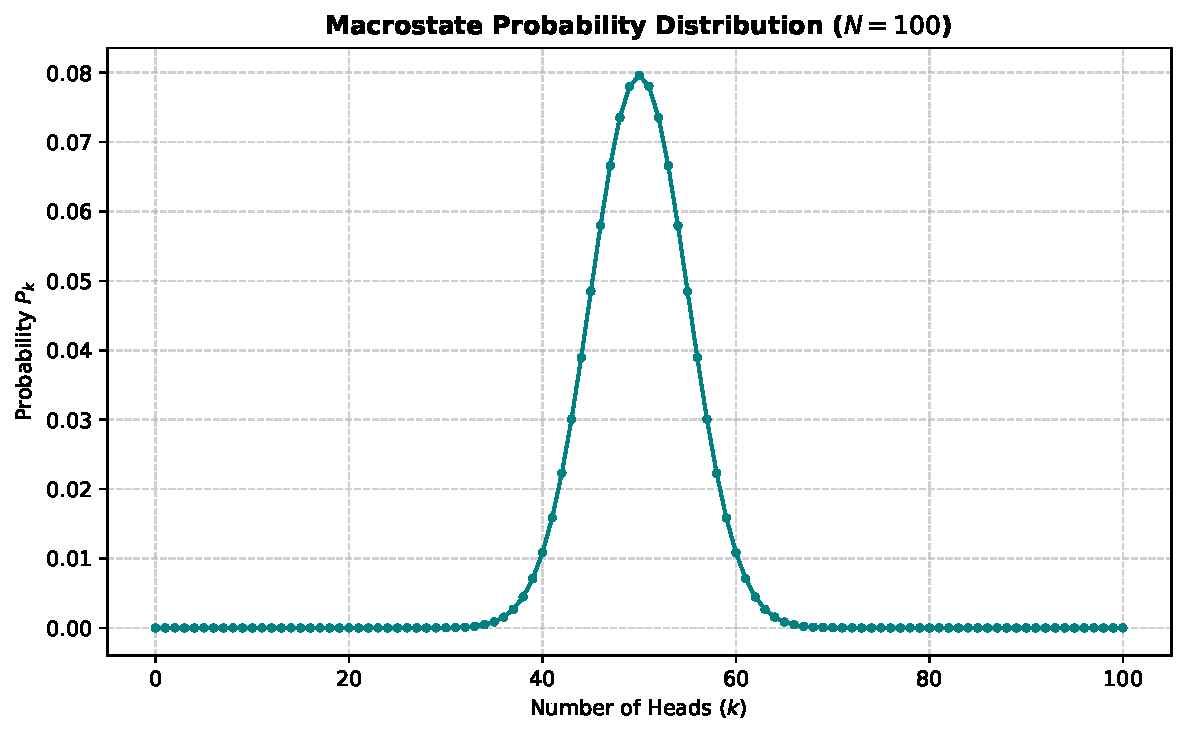
\includegraphics[width=\linewidth]{probability_distribution_N100.pdf}
    \end{minipage}

    \caption{Macrostate probability distributions for system sizes $N=20, 50, 80,$ and $100$.}
    \label{fig:macrostate_distributions}
\end{figure}

\subsection{Extrapolation to the Thermodynamic Limit}

As the system size is scaled up to the macroscopic limit $N \sim 10^{23}$, the characteristics of the macrostate distribution change drastically:

\textbf{Shape of the distribution.}
For any finite $N$, the probability distribution $P_k = \Omega(N,k)/2^N$ is a binomial distribution
centered at $\mu = N/2$ with standard deviation $\sigma = \sqrt{N}/2$. As we have experimentally proved with the previous plots and as it is shown by the Central Limit Theorem,
for large $N$ this converges to a Gaussian:
\begin{equation}
P_k \approx \sqrt{\frac{2}{\pi N}} \exp\!\left(-\frac{2(k - N/2)^2}{N}\right).
\end{equation}
The distribution maintains its bell shape, but its Variation Coefficient (VC), or relative width collapses:
\begin{equation}
\frac{\sigma}{\mu} = \frac{\sqrt{N}/2}{N/2} = \frac{1}{\sqrt{N}}.
\end{equation}
For a moderate $N$ (of the order of tens to hundreds of elements), fluctuations are small but visible. For $N \sim 10^{23}$, 
VC drops to $\sim 10^{-12}$, making any fluctuation from equilibrium almost
undetectable.

\textbf{Concentration of probabilities.}
As $N$ increases, the probability becomes more concentrated around $k = N/2.$ This means that the number of heads and tails will be almost equal in most cases. For a macroscopic system with $N \sim 10^{23}$, big differences between heads and tails will become extremely unlikely. In practice, the system will almost always remain very close to its most probable state..

\textbf{Entropy.}
The maximum entropy $S_{\max} = k_B \ln \Omega(N, N/2)$ grows with $N$. Using Stirling's approximation,
$\ln \Omega(N, N/2) \approx N \ln 2$, so $S_{\max} \approx N k_B \ln 2$, which scales proportionally to $N$, as expected. Therefore, the driving force of entropy toward
equilibrium  becomes increasingly strong as $N$ increases and large deviations will become highly unlikely.

\textbf{Spontaneous fluctuations.}
For small $N$, the probability of observing a highly ordered macrostate is small but nonzero, and the
expected waiting time to observe such a state, while large, is finite. For
$N \sim 10^{23}$, the probability of any macrostate deviating even a little bit from $N/2$ becomes so
small that the expected waiting time  exceeds any physically reasonable timescale. 

\textbf{Emergence of the Second Law.}
These results help explain the statistical origin of the Second Law of Thermodynamics. Since states with higher entropy are much more probable, an isolated system will naturally tend to evolve towards them. In small systems, occasional decreases in entropy can occur. However, for large macroscopic systems, decreases in entropy are so unlikely that the Second Law becomes absolute rule in practice.

\section{Probabilities, Entropy, and Thermodynamics}
All the tests performed in this section can be seen in \texttt{combinatorics\_tests.py} and

\texttt{thermodynamics\_tests.py}.
\subsection{Parameter Assignment}
The total number of coins in the system is defined as $N = 100 + M$, where $M$ is the harmonic mean of the last two digits of the four team members' unique academic identifiers (NIAs).

Given the last two digits for the four team members:
\begin{equation} x_1 = 7, \quad x_2 = 52, \quad x_3 = 12, \quad x_4 = 99 \end{equation}

The harmonic mean $M$ is calculated as follows:
\begin{equation} M = \frac{4}{\sum_{i=1}^{4} \frac{1}{x_i}} = \frac{4}{\frac{1}{7} + \frac{1}{52} + \frac{1}{12} + \frac{1}{99}} \end{equation}

Evaluating the sum of the reciprocals:
\begin{equation} \sum_{i=1}^{4} \frac{1}{x_i} \approx 0.142857 + 0.019231 + 0.083333 + 0.010101 = 0.255522 \end{equation}

Yielding the harmonic average:
\begin{equation} M = \frac{4}{0.255522} \approx 15.6542 \end{equation}

Rounding to the nearest integer gives $M = 16$. Consequently, the system parameters are established as:
\begin{equation} N = 100 + 16 = 116, \quad \text{and} \quad \frac{N}{2} = 58 \end{equation}

\subsection{Probability and Entropy Analysis}
Using the calculated $N = 116$, the probability of a specific macrostate $k$ is given by $P_k = \Omega(N,k)/2^N$. The calculated probabilities, cumulative distributions, and their statistical and thermodynamic interpretations are presented below:

\begin{enumerate}[label=\alph*)]
    \item \textbf{Probability of obtaining $k = 30$ heads:}
    \begin{equation} P(k = 30) = 6.355604 \times 10^{-8} \end{equation}
    Obtaining $k = 30$ heads lies more than $5.2$ standard deviations below the mean ($\mu = 58$, $\sigma = \frac{\sqrt{N}}{2} \approx 5.385$).
     The multiplicity $\Omega(116, 30)$ represents an infinitesimally small fraction ($\sim 0.0000064\%$) of the total $2^{116} \approx 8.307 \times 10^{34}$ microstates. Since entropy growss as $S = k_B \ln \Omega$, this state is highly ordered (low entropy), making spontaneous fluctuations to happen almost impossible without external work.
    

    \vspace{0.3cm}
    \item \textbf{Probability of obtaining $k = N/2$ heads (the most probable macrostate):}
    \begin{equation} P(k = 58) = 0.073922 \end{equation}
    
    $k = 58 = N/2$ is the expected value (mean and mode) of the symmetric distribution. It is the most probable macrostate among all 117 possible configurations ($k \in [0, 116]$).
    This represents \textbf{thermodynamic equilibrium}. Multiplicity reaches its absolute maximum here ($\Omega(116, 58) \approx 6.14 \times 10^{33}$), which maximizes system entropy ($S_{\text{max}} = k_B \ln \Omega_{\text{max}}$). Isolated physical systems evolve naturally toward this macrostate.
    

    \vspace{0.3cm}
    \item \textbf{Cumulative probability for $k_1 = N/2 - 10$ to $k_2 = N/2 + 10$ heads:}
    \begin{equation} \Delta P_{48, 68} = \sum_{k=48}^{68} P_k = 0.949270 \end{equation}
    An interval of $\pm 10$ heads around the mean ($\approx \pm 1.86\sigma$) accounts for $94.93\%$ of the total probability distribution.
    Demonstrates \textbf{concentration of measure}. Although $k \in [48, 68]$ spans only $18\%$ of accessible macrostates (21 of 117), nearly $95\%$ of all physical microstates reside inside this narrow central band, keeping thermal fluctuations tightly localized.
    

    \vspace{0.3cm}
    \item \textbf{Cumulative probability for $k_1 = N/2 - 20$ to $k_2 = N/2 + 20$ tails:}
    \begin{equation} \Delta P_{38, 78} = \sum_{k=38}^{78} P_k = 0.999880 \end{equation}
    Expanding the window to $\pm 20$ heads/tails ($\approx \pm 3.71\sigma$) encompasses $99.988\%$ of the probability space.
    Macrostates outside this interval ($k < 38$ or $k > 78$) have a combined probability of less than $0.012\%$. As $N \to \infty$, relative fluctuations $\frac{\sigma}{N} = \frac{1}{2\sqrt{N}} \to 0$, causing the probability density to collapse into a sharp delta function at equilibrium and illustrating why macroscopic violations of the Second Law of Thermodynamics are unobservable.
    
\end{enumerate}
\subsection{Entropy Change Analysis}
The entropy of a macrostate is defined as $S(k) = k_B \ln \Omega(N, k)$, where $k_B = 1.380649 \times 10^{-23}$ J/K is the Boltzmann constant. The entropy change between two macrostates $k_1$ and $k_2$ is computed as $\Delta S = S(k_1) - S(k_2) = k_B \bigl(\ln \Omega(N,k_1) - \ln \Omega(N,k_2)\bigr)$. The results for $N = 116$ are presented below:

\begin{enumerate}[label=\alph*)]
    \setcounter{enumi}{4}
    
    \item \textbf{Entropy change from $k_2 = N/2$ to $k_1 = N/2 + 25$:}
    \begin{equation} \Delta S = S(83) - S(58) = -1.5235 \times 10^{-22} \ \text{J/K} \approx -11.035 \, k_B \end{equation}
    Moving the system from maximum disorder ($k = 58$) to a highly ordered state ($k = 83$) requires a large entropy decrease. The negative sign means that, as expected, this transition is thermodynamically unfavourable: it would require external work to be performed on the system and cannot occur spontaneously in an isolated system.

    \vspace{0.3cm}
    \item \textbf{Entropy change from $k_2 = N/2$ to $k_1 = N/2 + 10$:}
    \begin{equation} \Delta S = S(68) - S(58) = -2.3717 \times 10^{-23} \ \text{J/K} \approx -1.718 \, k_B \end{equation}
    A displacement of $+10$ heads from the equilibrium produces a smaller but still negative entropy change. The macrostate $k = 68$ is still considerably probable to come out, far more probable than the macrostate $k = 83$, so this transition, although it is still unlikely to happen spontaneously, is far less unlikely than case~(e). 

    \vspace{0.3cm}
    \item \textbf{Entropy change from $k_2 = 20$ to $k_1 = N/2$:}
    \begin{equation} \Delta S = S(58) - S(20) = +3.7005 \times 10^{-22} \ \text{J/K} \approx +26.802 \, k_B \end{equation}
    Starting from a highly ordered state ($k = 20$, which lies $7.06\sigma$ below the mean) and evolving towards the most disordered case ($k = 58$) produces a large positive entropy change. This is a thermodynamically spontaneous process: the system gains entropy as it moves toward the most probable macrostate. The magnitude of the entropy change for this case is the largest out of the three of them, which is consistent with $k = 20$ being far more ordered than $k = 83$ and $k = 68$ and therefore having much fewer accessible microstates.
\end{enumerate}

\subsection{Thermodynamics Implications}
\begin{enumerate}[label=\alph*)]
    \setcounter{enumi}{7}
    
    \item \textbf{Time to highly ordered state ($k = 8$ heads):}
    \begin{equation} t = 1.1273 \times 10^{21} \ \text{s} \approx 3.5720 \times 10^{13} \ \text{years} \end{equation}
    Assuming a tossing rate of $N$ coins per second, the expected waiting time to randomly achieve this highly ordered state is incredibly large. To put this in perspective, this duration is orders of magnitude greater than the current age of the Universe. This illustrates very well the meaning of the Second Law of Thermodynamics: spontaneous macroscopic entropy decreases are not strictly impossible, but they are so extremely improbable that they are practically impossible to observe in practice.

    \vspace{0.3cm}
    \item \textbf{Likelihood ratio between the most probable state and $M \pm 10$ heads:}
    \begin{equation} \text{Ratio} = 5.5722 \end{equation} 
    This value quantifies how much more likely it is to obtain the equilibrium macrostate ($k = N/2$) compared to a more ordered configuration. A ratio of approximately $5.57$ shows that the system strongly favors the most disordered configuration, making even small macroscopic deviations from the mean (just 10 heads off) significantly less probable.
    
    \item \textbf{Second Law Interpretation:}

    
    None of the calculated results contradict the Second Law of Thermodynamics. From a statistical approach, isolated systems naturally evolve toward the macrostate with the highest uncertainty regarding its internal microscopic configuration, which corresponds to the state of maximum entropy. The Second Law does not state that spontaneous decreases in entropy are mathematically impossible, but rather that they are incredibly improbable. As demonstrated by the massive concentration of probability around the equilibrium state ($k = N/2$) and the absurdly long waiting times needed to randomly reach highly ordered configurations, macroscopic entropy decreases have a virtually zero chance of occurring. Therefore, these numerical results perfectly validate the nature of the Second Law instead of contradicting it.


    \item \textbf{Large $N$ Limit ($N \sim 10^{23}$):}
    Re-evaluating the system under the thermodynamic limit ($N \sim 10^{23}$) causes huge changes in its statistical behavior. As the number of particles approaches infinity, the relative fluctuations around the equilibrium state decay proportionally to $1/\sqrt{N}$. This scaling affects all previous calculations in the following ways:
    
    \begin{itemize}
        \item \textbf{Cumulative probability:} The cumulative probability distribution collapses entirely into an infinitely sharp Dirac delta peak exactly at the most probable macrostate ($k = N/2$). The probability of finding the system in any macroscopic state outside this strict equilibrium becomes practically zero.
        \item \textbf{Entropy change:} The entropy change ($\Delta S$) required to move the system away from maximum disorder (as seen in parts e and f) becomes an infinitely large negative value, meaning such transitions are strictly forbidden without massive external work. Conversely, the entropy gain when evolving toward equilibrium (part g) becomes infinitely large, driving a fully irreversible and deterministc spontaneous process.
        \item \textbf{Time to highly ordered state:} The expected waiting time to randomly achieve a highly ordered state diverges to infinity. It goes from being simply incredibly large to being absolutely impossible to observe.
        \item \textbf{Likelihood ratio:} The likelihood ratio between the equilibrium macrostate and any macrostate with a fixed macroscopic deviation tends to infinity. The macroscopic system is locked in the maximum entropy state.
    \end{itemize}
\end{enumerate}



\section{Conclusion}
In this practice, we successfully modeled the statistical mechanics of a binary system, demonstrating how the fundamental counting of microscopic configurations dictates macroscopic thermodynamic behavior. Through our computational analysis, we identified the strict physical and hardware limitations of full microstate enumeration. We observed an exponential time complexity barrier of $\mathcal{O}(2^N)$ that restricted our code execution to a maximum system size of $N = 26$ before computational time became impossible. 

By transitioning to analytical log-space combinatorics, we were able to evaluate a much larger system of $N = 116$ coins without suffering memory issues or numerical overflow. The results for this system confirmed an accurate localization of probability measure; specifically, $99.988\%$ of all possible microstates fall within a narrow fluctuation band of $\pm 20$ elements around the equilibrium mean of $58$ heads. 

Extrapolating these results to the true thermodynamic limit (as $N \to \infty$), the relative magnitude of these fluctuations approaches zero ($\frac{1}{2\sqrt{N}} \to 0$). This collapse of the probability density around the state of maximum multiplicity (and maximum entropy) confirms that spontaneous transitions to highly ordered, low-entropy macrostates are statistically negligible in large physical systems. Finally, our numerical results and analytical derivations successfully corroborate the fundamental statistical basis of the Second Law of Thermodynamics.

\appendix
\section{AI Collaboration \& Audit Statement}
In compliance with course policy, AI tools were utilized as code assistants. All generated algorithms were audited and validated using automated tests (\texttt{pytest}). Prompt logs and verification steps are recorded in \texttt{AI-STATEMENT.md} in the repository.

\end{document}